\documentclass{beamer}
\usepackage[utf8x]{inputenc}
\usepackage[ngerman]{babel}
\usepackage{amsmath}
\usepackage{amsfonts}
\usepackage{amssymb}
\usepackage{graphicx}
\usepackage{hyperref}
\usepackage{listings}
\lstset{literate=%
{Ö}{{\"O}}1
{Ä}{{\"A}}1
{Ü}{{\"U}}1
{ß}{{\ss}}2
{ü}{{\"u}}1
{ä}{{\"a}}1
{ö}{{\"o}}1
}

\lstset{language=C}

\author{Johannes Hackel \and Tim Illner \and Marcel Wesberg}
\title{OpenCL}

\usetheme{Ilmenau}
\useoutertheme{infolines}
\usecolortheme{rose}

\begin{document}

\begin{frame}
\titlepage
\end{frame}

\begin{frame}
\frametitle{Gliederung}
\tableofcontents
\end{frame}

\section{Was ist OpenCL?}
\begin{frame}[fragile]
\frametitle{Was ist OpenCL?}
%\url{http://en.wikipedia.org/wiki/OpenCL}
\end{frame}
\subsection{Geschichte}
\begin{frame}[fragile]
\frametitle{Geschichte}
%\url{http://en.wikipedia.org/wiki/OpenCL#History}
\end{frame}
\subsection{Unterstütze Geräte/Treiber}
\begin{frame}[fragile]
\frametitle{Unterstütze Geräte/Treiber}
%\url{http://en.wikipedia.org/wiki/OpenCL#OpenCL-conformant_products}
\end{frame}

\section{Aufbau GPUs}
\begin{frame}[fragile]
\frametitle{Aufbau GPUs}
\begin{itemize}
\item Grafikprozessor besteht aus Recheneinheiten, ähnlich CPU:
\item Ausführung Operationen der Arithmetik, Decodierung und Datentransfer
\item Verarbeitung paralleler Prozesse (zB. mathematischer Operationen) bei konstanter Taktrate
\item Durch breiten Datenbus mit Speichereinheit verbunden, großer Datendurchsatz
\item Verarbeitung vieler Daten gleichzeitig:
\item graphische, dreidimensionale Objekte, Beleuchtung, Farben und Texturen
\item Auswertung wissenschaftliche Daten
\item Simulation komplexer physikalischer Systeme (zB. viele kleine Teilchen)
\end{itemize}
\end{frame}

\begin{frame}[fragile]
\begin{figure}
\begin{center}
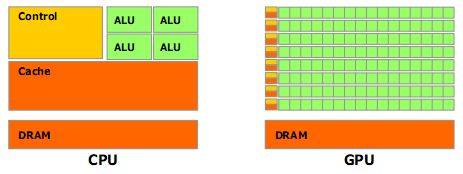
\includegraphics[width=10cm]{cpu_gpu.png}
\end{center}
\end{figure}
\end{frame}

\section{Die OpenCL}
\subsection{Kernel}
\begin{frame}[fragile]
\frametitle{Die OpenCL}
\framesubtitle{Kernel}
\begin{lstlisting}
float Sum(float x, float y)
{
 return(x + y);
}

__kernel void Calculate(__global float* input,
 __global float* output)
{
 
}
\end{lstlisting}
\end{frame}

\subsection{Datentypen}
\begin{frame}[fragile]
\frametitle{einfache Datentypen}
\begin{itemize}

\item bool: Boolescher Wahrheitswert, true oder false.
\item char: Vorzeichenbehaftete 8-Bit Ganzzahl.
\item uchar, unsigned char: Vorzeichenlose 8-Bit Ganzzahl.
\item short: Vorzeichenbehaftete 16-Bit Ganzzahl.
\item ushort, unsigned short: Vorzeichenlose 16-Bit Ganzzahl.
\item int: Vorzeichenbehaftete 32-Bit Ganzzahl.
\item uint, unsigned int: Vorzeichenlose 32-Bit Ganzzahl.
\item long: Vorzeichenbehaftete 64-Bit Ganzzahl.
\item ulong, unsigned long: Vorzeichenlose 64-Bit Ganzzahl.
\item float: 32-Bit Gleitkommazahl.
\item half: 16-Bit Gleitkommazahl.

\end{itemize}
\end{frame}

\begin{frame}[fragile]
\frametitle{Vektordatentypen}
\begin{itemize}
\item bestehend aus 2, 3, 4, 8 oder 16 Elementen
\item vom Typ char, uchar, short, ushort, int, uint, long, ulong oder float
\item verschiedene Möglichkeiten der Deklaration und Initialisierung
\end{itemize}
\begin{lstlisting}
float4 a = (float4)(0.0, 1.0, 2.0, 3.0);
float2 b = (float2)(1.0, 2.0);
float2 c = (float2)(0.0);
float4 d = (float4)(b, c);
float8 e = (float8)(b, a, c);
\end{lstlisting}
\end{frame}

\begin{frame}[fragile]
\frametitle{Vektordatentypen}
\begin{itemize}
\item Komponentenweise Addition, Subtraktion und Multiplikation:
\end{itemize}
\begin{lstlisting}
float4 a, b, c;
int8 d, e, f, g;
c = a + b;
c = a - b;
f = d * e;
g = 2 * f;
\end{lstlisting}
\end{frame}

\begin{frame}[fragile]
\frametitle{Vektordatentypen}
\begin{large}
Zugriff auf einzelne Komponenten:
\end{large}
\\
\begin{itemize}
\item  bei 2, 3 oder 4 Elementen durch x, y, z, w
\item bei 8 Elementen: s0 bis s7
\item bei 16 Elementen: s0 bis s9 und sa bis sf
\end{itemize}
\begin{lstlisting}
float4 a;
float b = a.z;
float c = a.s2;
float16 d;
float e = d.sf;
float2 f, g;
float8 h;
float16 i;
g.xy = f.yx;
g.s01 = f.s10;
h.s01234567 = i.sfedcba98;
\end{lstlisting}
\end{frame}


\subsection{Speicherbereiche}
\begin{frame}[fragile]
\frametitle{Speicherbereiche}
\begin{center}
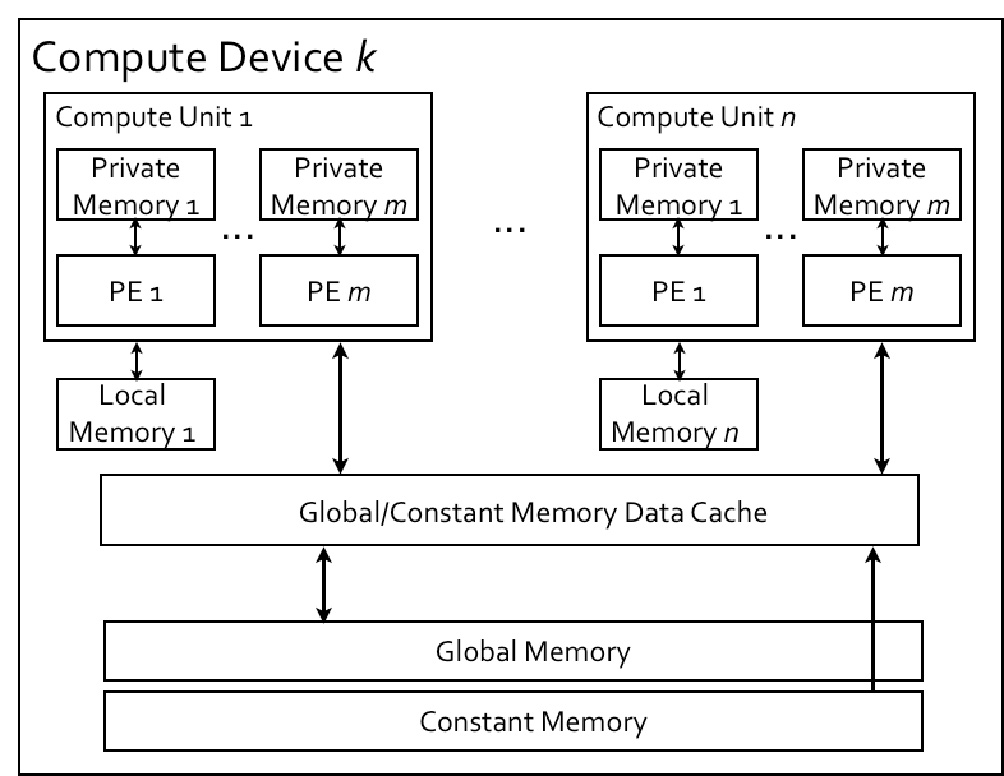
\includegraphics[width=10cm]{opencl_memory.jpg}
\end{center}
\end{frame}

\begin{frame}[fragile]
\frametitle{Speicherbereiche}
privater Speicher:
\begin{itemize}
\item \_\_private
\item Variablen die in einer Funktion deklariert wurden und Funktionsargumente
\item nur in dieser Funktion zugänglich
\item existieren nur für die jeweilige Kernel-Instanz
\end{itemize}
lokaler Speicher:
\begin{itemize}
\item \_\_local
\item werden von allen Kernel-Instanzen in einer Arbeitsgruppe gemeinsam genutzt
\item jede Arbeitsgruppe besitzt eigene Kopie 
\end{itemize}
\end{frame}

\begin{frame}[fragile]
\frametitle{Speicherbereiche}
globaler Speicher:
\begin{itemize}
\item \_\_global
\item Zugriff von Host und Client möglich
\item üblicherweise ein Zeiger auf Speicherbereich
\item alle Kernel-Instanzen greifen auf die selben Daten zu
\end{itemize}
Konstantenspeicher:
\begin{itemize}
\item \_\_constant
\item nur lesbar
\item kann in lokalen Speicher liegen
\end{itemize}
\end{frame}

\subsection{Funktionen}
\begin{frame}[fragile]
\frametitle{Funktionen für die Arbeitsverwaltung}
\begin{itemize}
\item uint get\_work\_dim(void)
\item size\_t get\_global\_size(uint dim)
\item size\_t get\_global\_id(uint dim)
\item size\_t get\_local\_size(uint dim)
\item size\_t get\_local\_id(uint dim)
\item size\_t get\_num\_groups(uint dim)
\item size\_t get\_group\_id(uint dim)
\item size\_t get\_global\_offset(uint dim)
\end{itemize}
\end{frame}


\begin{frame}[fragile]
\frametitle{Mathematische Funktionen}
\begin{itemize}
\item Exponentialfunktion und Logarithmus: exp, exp2, exp10, log, log2, log10
\item Trigonometrische Funktionen: sin, cos, tan, asin, acos, atan, atan2
\item Hyperbolische Funktionen: sinh, cosh, tanh, asinh, acosh, atanh
\item Wurzeln: sqrt, cbrt
\item Potenzen: pow
\item Rundungsfunktionen: round, floor, ceil
\item weiter Funktionen findet man in der OpenCL-Spezifikation
\end{itemize}
\end{frame}

\section{Die Laufzeitbibliotheken}
\begin{frame}[fragile]
\frametitle{Die Laufzeitbibliotheken}
\begin{figure}
\begin{center}
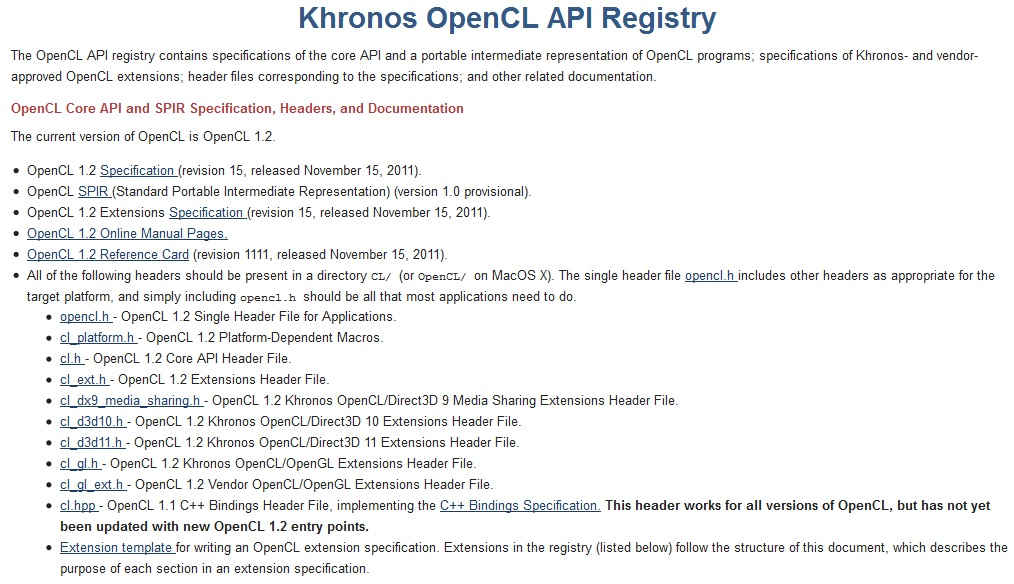
\includegraphics[width=10cm]{Khronos_API_page.jpg}
\end{center}
\end{figure}
Eine Übersicht der verfügbaren Laufzeitbibliotheken erhält man auf
\url{http://www.khronos.org/registry/cl/}
\end{frame}

\subsection{Plattformen/Geräte}
\begin{frame}[fragile]
\frametitle{Plattformen}
\begin{lstlisting}
clGetPlatformIDs(cl_uint       /* num_entries */,
 cl_platform_id * /* platforms */,
 cl_uint *        /* num_platforms */);


clGetPlatformInfo(cl_platform_id   /* platform */, 
 cl_platform_info /* param_name */,
 size_t           /* param_value_size */, 
 void *           /* param_value */,
 size_t *         /* param_value_size_ret */);
\end{lstlisting}
\end{frame}

\begin{frame}[fragile]
\frametitle{Geräte}
\begin{lstlisting}
clGetDeviceInfo(cl_device_id    /* device */,
 cl_device_info  /* param_name */, 
 size_t          /* param_value_size */, 
 void *          /* param_value */,
 size_t *        /* param_value_size_ret */);


clCreateSubDevices(cl_device_id      /* in_device */,
 const cl_device_partition_property* /* properties*/,
 cl_uint             /* num_devices */,
 cl_device_id *      /* out_devices */,
 cl_uint *           /* num_devices_ret */);
\end{lstlisting}
\end{frame}

\subsection{Kontexte/Speicherverwaltung}
\begin{frame}[fragile]
\frametitle{Kontexte}
\begin{lstlisting}
clGetContextInfo(cl_context    /* context */, 
 cl_context_info    /* param_name */, 
 size_t             /* param_value_size */, 
 void *             /* param_value */, 
 size_t *           /* param_value_size_ret */);
\end{lstlisting}
\end{frame}

\begin{frame}[fragile]
\frametitle{Speicherverwaltung}
\begin{lstlisting}
clGetMemObjectInfo(cl_mem      /* memobj */,
 cl_mem_info      /* param_name */, 
 size_t           /* param_value_size */,
 void *           /* param_value */,
 size_t *         /* param_value_size_ret */);

clEnqueueWriteBuffer(
cl_command_queue /* command_queue */,
 cl_mem   /* buffer */,
 cl_bool  /* blocking_write */, size_t  /* offset */,
 size_t    /* size */, const void *   /* ptr */, 
 cl_uint            /* num_events_in_wait_list */, 
 const cl_event *   /* event_wait_list */, 
 cl_event *         /* event */);
\end{lstlisting}
\end{frame}

\subsection{Programme/Kernels}
\begin{frame}[fragile]
\frametitle{Programme}
\begin{lstlisting}
clGetProgramBuildInfo(cl_program    /* program */,
 cl_device_id          /* device */,
 cl_program_build_info /* param_name */,
 size_t                /* param_value_size */,
 void *                /* param_value */,
 size_t *              /* param_value_size_ret */);
\end{lstlisting}
\end{frame}

\begin{frame}[fragile]
\frametitle{Programme}
\begin{lstlisting}
clCompileProgram(cl_program        /* program */,
 cl_uint              /* num_devices */,
 const cl_device_id * /* device_list */,
 const char *         /* options */, 
 cl_uint              /* num_input_headers */,
 const cl_program *   /* input_headers */,
 const char **        /* header_include_names */,
 void (CL_CALLBACK *  /* pfn_notify */)
 (cl_program /* program */,void * /* user_data */),
 void *               /* user_data */);
\end{lstlisting}
\end{frame}

\begin{frame}[fragile]
\frametitle{Kernel}
\begin{lstlisting}
clCreateKernelsInProgram(cl_program  /* program */,
              cl_uint        /* num_kernels */,
              cl_kernel *    /* kernels */,
              cl_uint *      /* num_kernels_ret */);


clSetKernelArg(cl_kernel    /* kernel */,
               cl_uint      /* arg_index */,
               size_t       /* arg_size */,
               const void * /* arg_value */);
\end{lstlisting}
\end{frame}

\subsection{Warteschlangen/Ereignisse/Marker und Barrieren}
\begin{frame}[fragile]
\frametitle{Warteschlangen}
\begin{lstlisting}
clCreateCommandQueue(cl_context      /* context */, 
                     cl_device_id   /* device */, 
    cl_command_queue_properties    /* properties */,
                     cl_int *     /* errcode_ret */);


clEnqueueReadBuffer(
 cl_command_queue    /* command_queue */,
 cl_mem   /* buffer */, cl_bool  /* blocking_read */,
 size_t   /* offset */, size_t   /* size */, 
 void *   /* ptr */,
 cl_uint  /* num_events_in_wait_list */,
 const cl_event *    /* event_wait_list */,
 cl_event *          /* event */);
\end{lstlisting}
\end{frame}

\begin{frame}[fragile]
\frametitle{Ereignisse}
\begin{lstlisting}
clWaitForEvents(cl_uint  /* num_events */,
 const cl_event *    /* event_list */);


clGetEventInfo(cl_event         /* event */,
 cl_event_info    /* param_name */,
 size_t           /* param_value_size */,
 void *           /* param_value */,
 size_t *         /* param_value_size_ret */);


clCreateUserEvent(cl_context    /* context */,
 cl_int *      /* errcode_ret */)
\end{lstlisting}
\end{frame}

\begin{frame}[fragile]
\frametitle{Marker und Barrieren}
\begin{lstlisting}
clEnqueueMarker(
   cl_command_queue  /* command_queue */,
   cl_event *        /* event */);



clEnqueueBarrier(
   cl_command_queue /* command_queue */)
\end{lstlisting}
\end{frame}

\section{Kompilierung und Ausführung}
\begin{frame}[fragile]
\frametitle{Kompilierung und Ausführung}
\end{frame}

\section{Quellen}
\begin{frame}[fragile]
\frametitle{Quellen}
\begin{itemize}
\item \url{http://www.khronos.org/}
\item \url{hexagon.fi.tartu.ee/~manuel/teaching/gpu.pdf}
\item \url{http://www.zdnet.de/wp-content/uploads/legacy_images/news/201004/aws-gpu-v6.png}
\item \url{http://developer.amd.com/Resources/documentation/articles/PublishingImages/opencl_figure5.jpg}
\end{itemize}
\end{frame}
\end{document}